\PassOptionsToPackage{dvipsnames}{xcolor}
\documentclass[mathserif]{beamer}

\usepackage{tgadventor}
\usepackage[absolute,overlay]{textpos}

\usepackage{listings}
\definecolor{light-gray}{gray}{0.9}
\lstset{columns=fullflexible, 
        basicstyle=\ttfamily\footnotesize,
        breaklines=true,
        backgroundcolor=\color{light-gray},
        xleftmargin=0.5cm,
        frame=tlbr,
        framesep=4pt,
        framerule=0pt}


% approx symbol
\usepackage{textcomp}
\newcommand{\textapprox}{\raisebox{0.5ex}{\texttildelow}}

\addtobeamertemplate{title page}{\center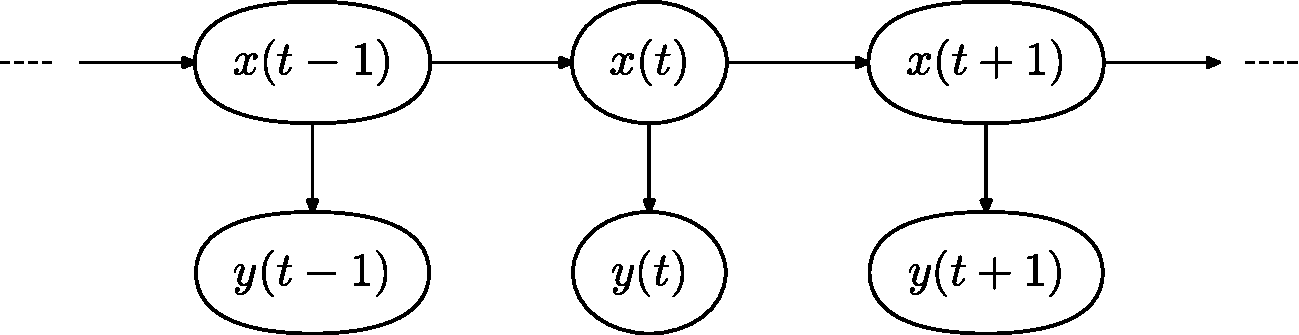
\includegraphics[scale=.4]{figures/Hmm_temporal_bayesian_net.pdf}\\\medskip}{}

\title{Specifying Graphical Models in \texttt{RevBayes}}
\author{Will Freyman}
\institute{
  Department of Ecology, Evolution \& Behavior \\
  University of Minnesota \\
  \medskip
  \color{Emerald}willfreyman@gmail.com \\
  http://willfreyman.org

}
\date{UC Berkeley Workshop, February 26-27 2018}


\beamertemplatenavigationsymbolsempty

\setbeamercolor{alerted text}{fg=Emerald}


\begin{document}


\frame{\titlepage}

\begin{frame}
    \begin{block}{Workshop goals:}
    \begin{itemize}
        \item not simply demonstrate ``standard'' phylogenetic analyses in \texttt{RevBayes}
        \item instead we'll explore the flexibility of a graphical modeling framework 
        \item use graphical models to see how the models underlying tree inference and downstream tree use (comparative methods) are linked
        \item enable participants to specify custom and unique phylogenetic analyses in \texttt{RevBayes}
    \end{itemize}
    \end{block}
\end{frame}


\begin{frame}
    \begin{block}{What are we doing in phylogenetics?}
    \begin{itemize}
        \item ``inference''? (i.e. statistical inference?)
        \item ``learning''? (i.e. machine learning?)
        \item ``prediction''?
    \end{itemize}
    \bigskip
        In a probabilistic framework (maximum likelihood or Bayesian) 
        inference and learning are the same\\
    \bigskip
        When we ``train'' a machine learning algorithm we are doing parameter estimation\\
    \bigskip
        The field of machine learning includes camps that use principled probabilistic approaches and camps that use heuristic ad hoc methods (like in phylogenetics!)\\
    \bigskip
        In phylogenetics we should be doing more \alert{prediction}! \\
    i.e. model adequacy/posterior predictive tests
    \end{block}
\end{frame}


\begin{frame}
    \begin{block}{What is a model?}
    \begin{itemize}
        \item in statistics?
        \item in machine learning?
        \item in biology?
    \end{itemize}
    \end{block}
    \begin{block}{maybe:}
    \begin{itemize}
     \item a way to relate data to hypotheses?
        \begin{itemize}
            \item what about heuristic or ad hoc approaches? 
            \item is parsimony in phylogenetics a model, an algorithm, or a philosophy?
        \end{itemize}
     \item a set of assumptions about the data-generating process?
     \item ``a formal representation of a theory''?
     \item a set of mathematical equations that relate one or more random variables?
    \end{itemize}
    \end{block}
\end{frame}


\begin{frame}
    \begin{block}{The distinction between models and algorithms:}
    \bigskip
    \begin{tabular}{ c | c }
        model & algorithm \\
        \hline
        phylogenetic models & pruning algorithm \\
        Bayesian graphical model & belief propagation \\
        neural networks & backpropagation \\
        Hidden Markov model &  forward-backward \\
        k-means clustering &  Lloyd's algorithm \\
        linear regression & least-squares \\
    \end{tabular} \\
    \bigskip
        Learning algorithms typically either optimize $\hat{\theta}$ or integrate to infer $p(\theta|D)$ \\
    \bigskip
        They are often \textit{very similar} and can be used with other models \\
    \bigskip
        Any well defined model can be treated in a \textit{probabilistic} framework and
        then we can use Bayesian \alert{or} maximum likelihood approaches
    \end{block}
\end{frame}


\begin{frame}
        \small
    \begin{block}{Probabilistic models:}
        \bigskip
        Instead of a hodgepodge of different heuristic methods
        these models use the principles of probability theory \\
        \bigskip
        Why use them?
        \begin{itemize}
            \item Quantify uncertainty: they know when they don't know
                \begin{itemize}
                    \item what is the best prediction/decision/inference given data? 
                    \item what is the best model/hypothesis given the data? 
                    \item do I need more/different data? 
                \end{itemize}
            \item natural complexity control 
                \begin{itemize}
                    \item preventing overfitting / regularization
                \end{itemize}
            \item modularity
                \begin{itemize}
                    \item models as ``lego kits''
                    \item different inferential algorithms can use the same model
                    \item different models can use the same inferential algorithm
                \end{itemize}
        \end{itemize}
    \end{block}
\end{frame}



\begin{frame}
\small
    \frametitle{Discriminative vs Generative Models}
    \begin{block}{Discriminative (or conditional) models:}
    \begin{enumerate}
        \item models a response variable conditioned on a predictor variable
        \item models the conditional distribution $p(y|x)$
        \item makes fewer assumptions about the data: $p(x)$ not necessary
    \end{enumerate}
    \end{block}
    \begin{block}{Phylogenetic examples:} 
    \begin{itemize}
        \item estimating divergence times over a fixed topology
        \item estimating ancestral states on a fixed tree
        \item estimating shifts in diversification rates over a fixed tree
    \end{itemize}
    \end{block}
\end{frame}
\begin{frame}
\small
    \frametitle{Discriminative vs Generative Models}
    \begin{block}{Generative models:}
    \begin{enumerate}
        \item models the entire process used to generate the data
        \item models the joint distribution $p(x, y)$
        \item makes more assumptions about the data: need to define $p(x)$ 
        \item richer representation of the relations between variables
        \item more powerful: allows us to compute $p(y|x)$ or $p(x|y)$ 
        \item more powerful: can simulate both $x$ and $y$
    \end{enumerate}
    \end{block}
    \begin{block}{Phylogenetic examples:} 
    \begin{itemize}
        \item jointly estimating divergence times and the tree topology
        \item jointly estimating ancestral states and the tree
        \item jointly estimating shifting diversification rates and the tree
    \end{itemize}
    \end{block}
\end{frame}



\begin{frame}

    \frametitle{What is a graphical model?}
    \small
    \begin{block}{Also called:}
    \begin{enumerate}
        \item Bayesian networks
        \item belief networks
        \item causal networks
    \end{enumerate}
    \end{block}
    \begin{block}{A useful way to represent a probabilistic model: a joint distribution of random variables.}
    \end{block}
    We can specify both generative and discriminative models as graphical models. 
\end{frame}


\begin{frame}

    \frametitle{What is a graphical model?}
    \small
    \begin{block}{Nodes represent variables and edges represent conditional dependencies:}
    \begin{center}
    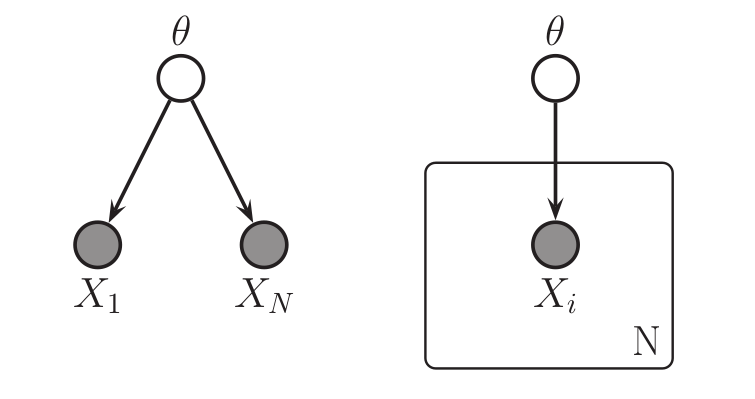
\includegraphics[scale=0.3]{figures/graphical_model.png}\\
        \medskip
        $p(\theta,\mathcal{D}) = p(\theta) \Big[ \displaystyle\sum^N_{i=1} p(x_i|\theta) \Big]$
    \end{center}
    \end{block}
    \begin{textblock*}{10cm}(1cm,9cm)
    \tiny Image from Murphy (2012)
    \end{textblock*}
\end{frame}


\begin{frame}

    \frametitle{What is a graphical model?}
    \small
    \begin{center}
    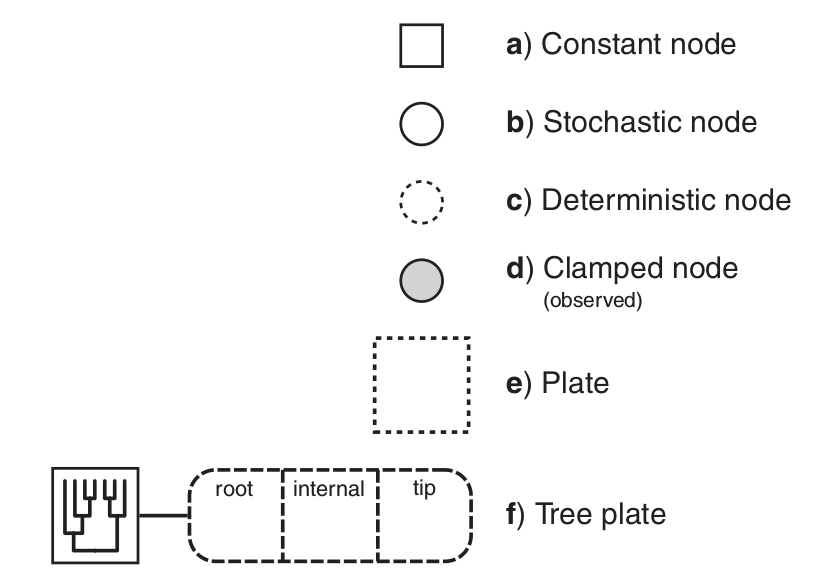
\includegraphics[scale=0.3]{figures/graphical_model_legend.png}\\
    \end{center}
    \begin{textblock*}{10cm}(1cm,9cm)
    \tiny Image from H\"oehna et al. (2014)
    \end{textblock*}
\end{frame}

\begin{frame}

    \small
    \begin{center}
    \alert{phylogenetic graphical model}
    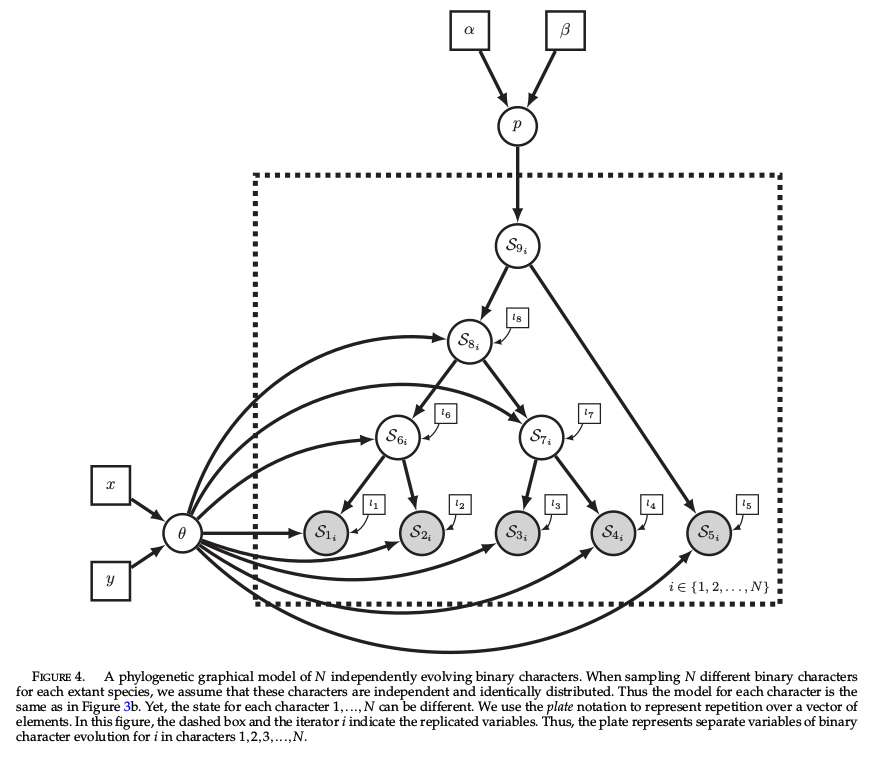
\includegraphics[scale=0.3]{figures/phylo_graphical.png}\\
    \end{center}
    \begin{textblock*}{10cm}(1cm,9.2cm)
    \tiny Image from H\"oehna et al. (2014)
    \end{textblock*}
\end{frame}


\begin{frame}

    \small
    \begin{center}
    \alert{phylogenetic graphical models as modules}\\
    \bigskip
    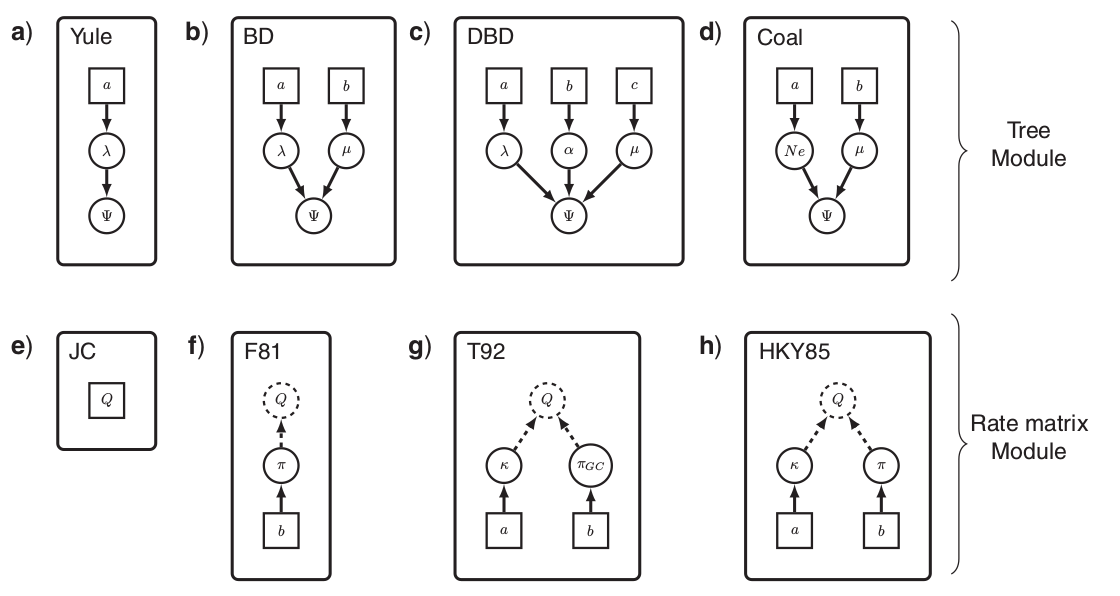
\includegraphics[scale=0.3]{figures/graphical_modular.png}\\
    \end{center}
    \begin{textblock*}{10cm}(1cm,9cm)
    \tiny Image from H\"oehna et al. (2014)
    \end{textblock*}
\end{frame}


\begin{frame}
    \small
    \begin{center}
    \alert{assembling phylogenetic models like lego kits}\\
    \bigskip
    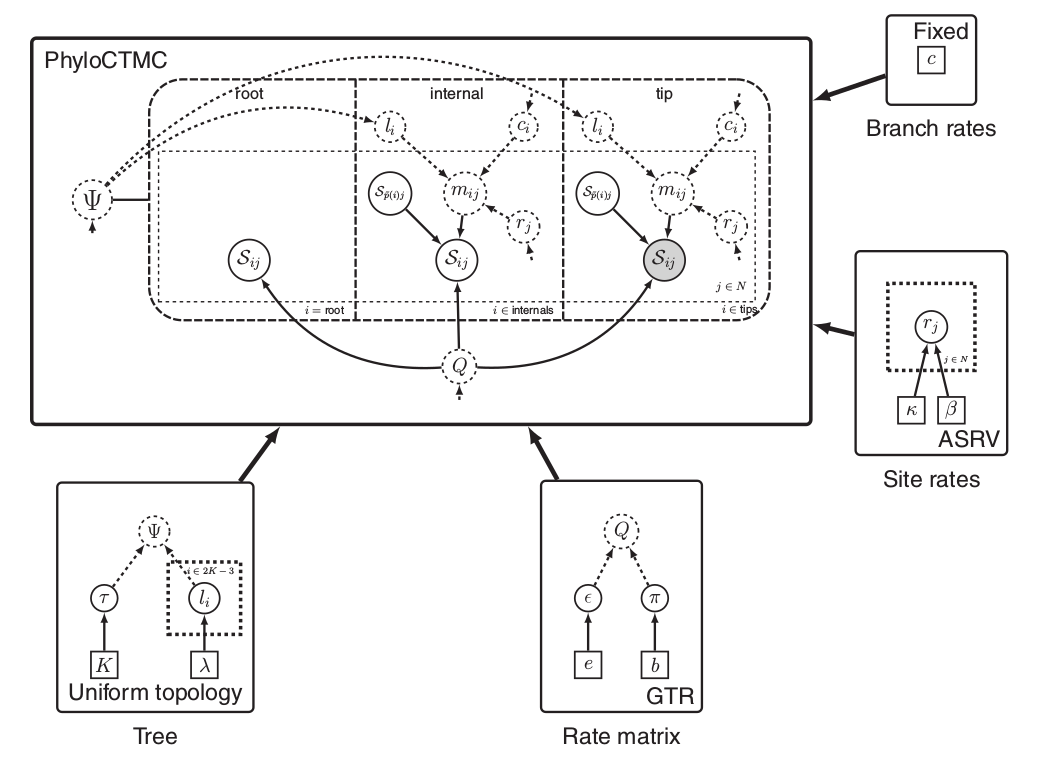
\includegraphics[scale=0.3]{figures/graphical_lego_kit.png}\\
    \end{center}
    \begin{textblock*}{10cm}(1cm,9.2cm)
    \tiny Image from H\"oehna et al. (2014)
    \end{textblock*}
\end{frame}


\begin{frame}
    \begin{block}{Is the graphical model paradigm really helpful?}
    \bigskip
    \small
    Disadvantages: 
    \begin{enumerate}
        \item steep learning curve...
        \begin{itemize}
            \item constant, stochastic, deterministic nodes
            \item clamping
            \item MCMC proposals
        \end{itemize}
    \end{enumerate}
    Advantages: 
    \begin{enumerate}
        \item transparency: all modeling assumptions are specified
        \item power and flexibility: build custom models that test your specific hypotheses 
        \item efficiency: customize inference algorithm to efficiently perform inference 
        \item applicability: the same concepts are widely used in many probabilistic programming languages like Stan, BUGS, Edward, PyMC3... and \texttt{Rev}!
    \end{enumerate}
    \end{block}
\end{frame}


\begin{frame}

    \small
    \begin{block}{The \texttt{Rev} probabilistic programming language:}
    \bigskip
    Most \texttt{Rev} scripts have two important aspects woven together: 
    \begin{enumerate}
        \item the graphical model specification
        \item the inference algorithm specification (MCMC moves, etc.)
    \end{enumerate}
    Since our goal is think abstractly in terms of graphical models
     we're going to learn these two aspects separately. \\
     \bigskip
        In \texttt{Rev} we can specify any type of probabilistic model, not just phylogenetic models:
    \begin{itemize}
        \item classification models
        \item time series models
        \item neural networks
        \item etc...
    \end{itemize}
    \end{block}
\end{frame}


\begin{frame}
    \small
    \begin{center}
    \alert{linear regression as a graphical model}\\
    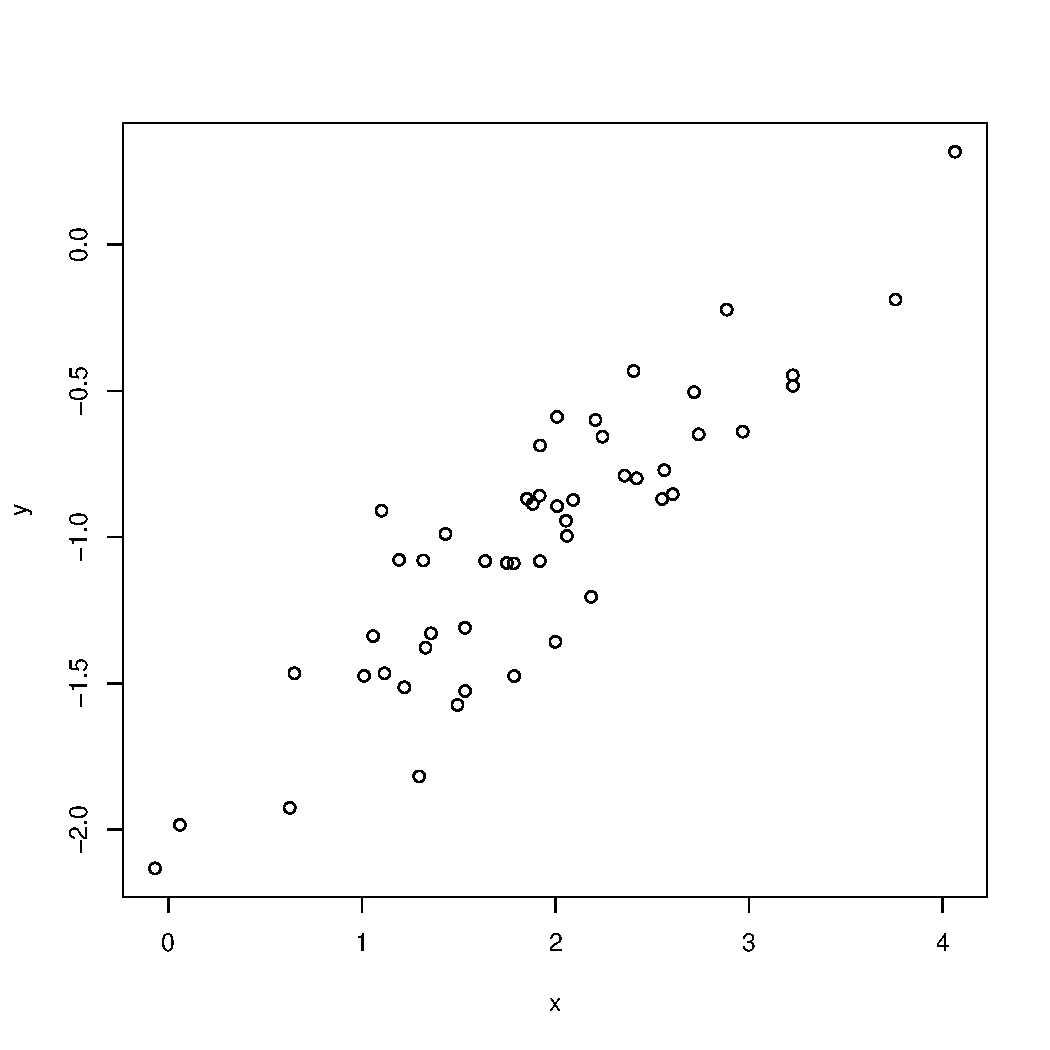
\includegraphics[scale=0.4]{figures/linear_regression.pdf}\\
    \smallskip
    $y = \beta x + \alpha + \epsilon$\\
    \end{center}
\end{frame}

\begin{frame}
    \small
    \begin{center}
    \alert{linear regression as a graphical model}\\
    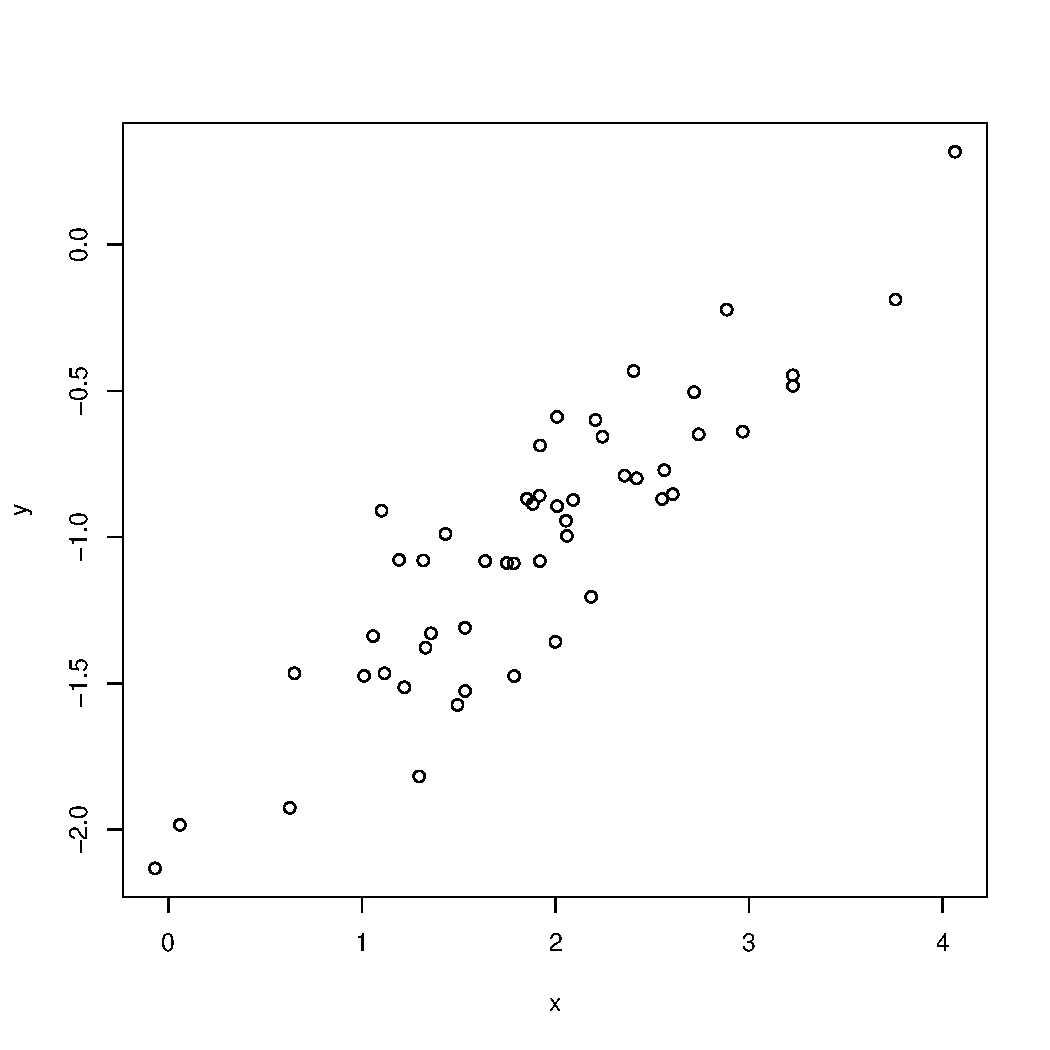
\includegraphics[scale=0.4]{figures/linear_regression.pdf}\\
    \smallskip
    $\mu_y = \beta x + \alpha$\\
    $y \sim \text{Normal}(\mu_y, \sigma_{\epsilon})$\\
    \end{center}
\end{frame}


\begin{frame}
    \small
    \begin{center}
    \alert{Bayesian linear regression}\\
    \bigskip
    \bigskip
    $\mu_y = \beta x + \alpha$\\
    $y \sim \text{Normal}(\mu_y, \sigma_{\epsilon})$\\
    \bigskip
    \bigskip
    We need some priors!\\
    \bigskip
    \bigskip
    $\beta \sim \text{Normal}(\mu=0, \sigma^2=1)$\\
    $\alpha \sim \text{Normal}(\mu=0, \sigma^2=1)$\\
    $\sigma_{\epsilon} \sim \text{Exponential}(\lambda=1)$\\
    \end{center}
\end{frame}

\begin{frame}[fragile]
Now let's program the model in \texttt{Rev}...\\
    \bigskip
    First clone the workshop's repo and start \texttt{rb}:\\
    \bigskip
    \begin{lstlisting}
git clone https://github.com/wf8/RevBayes_UC_Berkeley_2018_Workshop.git
cd RevBayes_UC_Berkeley_2018_Workshop
rb
    \end{lstlisting}
\bigskip
    The full example scripts are in the \texttt{src/} directory, but instead of using \texttt{source()}
    let's walk through the script interactively...
\end{frame}

\begin{frame}[fragile]
    Our observed data are constant nodes:\\
    \bigskip
    \begin{lstlisting}
x_obs <- readDataDelimitedFile(file="data/x.csv", header=FALSE, delimiter=",")[1]
y_obs <- readDataDelimitedFile(file="data/y.csv", header=FALSE, delimiter=",")[1]
    \end{lstlisting}
\bigskip
    Take a look at \texttt{x\_obs} and \texttt{y\_obs}: they are simply vectors containing these points:\\
    \center
    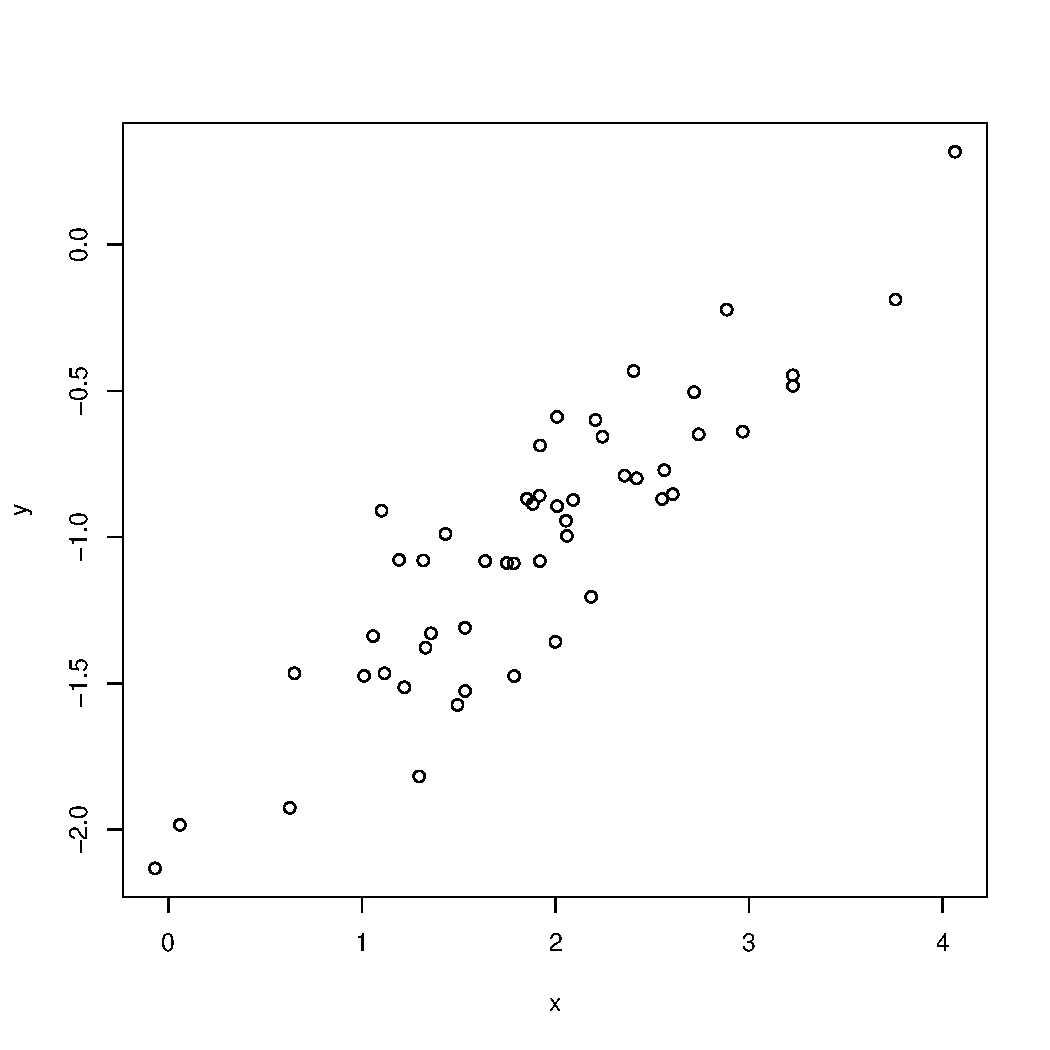
\includegraphics[scale=0.2]{figures/linear_regression.pdf}\\
\end{frame}


\begin{frame}[fragile]
    We'll specify relatively uninformative priors for our parameters. These are stochastic nodes:\\
    \bigskip
    \begin{lstlisting}
beta ~ dnNormal(0, 1)
alpha ~ dnNormal(0, 1)
sigma ~ dnExponential(1)
    \end{lstlisting}
\end{frame}


\begin{frame}[fragile]
And now deterministic nodes for $\mu_y$ and stochastic nodes for $y$:\\
    \bigskip
    \begin{lstlisting}
for (i in 1:x_obs.size()) {
    mu_y[i] := (beta * x_obs[i]) + alpha
    y[i] ~ dnNormal(mu_y[i], sigma)
}
    \end{lstlisting}
\bigskip
    We have now simulated values of $y$ conditioned on $x$. 
    So this is a \alert{discriminative} model.  \\
\bigskip
What happens if we set the value of $\beta$ or $\alpha$ to something else?
    Try the \texttt{setValue()} and \texttt{redraw()} member methods.
\end{frame}


\begin{frame}[fragile]
To estimate parameter values, we need to \alert{clamp}
the observed values of $y$:
    \bigskip
    \begin{lstlisting}
for (i in 1:x_obs.size()) {
    mu_y[i] := (beta * x_obs[i]) + alpha
    y[i] ~ dnNormal(mu_y[i], sigma)
    y[i].clamp(y_obs[i])
}

mymodel = model(beta)
    \end{lstlisting}
\bigskip
    So now we have specified the full linear regression model in a \alert{discriminative} form: $y$ conditioned on $x$.  \\
\bigskip
Let's set up the MCMC...
\end{frame}


\begin{frame}[fragile]
We need at least one MCMC move for each parameter we want to estimate:
    \bigskip
    \begin{lstlisting}
moves[1] = mvSlide(beta)
moves[2] = mvSlide(alpha)
moves[3] = mvSlide(sigma)
    \end{lstlisting}
\bigskip
We also need monitors for the MCMC:
    \bigskip
    \begin{lstlisting}
monitors[1] = mnScreen()
monitors[2] = mnModel("output/linear_regression.log")
    \end{lstlisting}
\end{frame}


\begin{frame}[fragile]
Now run the MCMC:
    \bigskip
    \begin{lstlisting}
mymcmc = mcmc(mymodel, moves, monitors)
mymcmc.run(10000)
    \end{lstlisting}
\bigskip
Look at the results in Tracer. What estimates do you get for $\alpha$, $\beta$, and $\sigma$?\\
    \bigskip
The true values were $\alpha = -2$, $\beta = 0.5$, and $\sigma = 0.2$.\\
    \bigskip
    \bigskip
    \alert{Exercise:} modify this to be a fully \alert{generative} model.\\
    \bigskip
    \alert{Exercise:} experiment with different MCMC moves to make the analysis converge more efficiently.
\end{frame}


\begin{frame}
    \begin{block}{Finally phylogenetics!}
        \bigskip
        Let's use the distinction between a \alert{discriminative} (or conditional) model and
        a \alert{generative} model to explore the link between tree inference models
        and comparative methods....
    \end{block}
\end{frame}

% walk through discriminative model script

% exercise: modify this to make the model fully generative


% walk through setting up MCMC for this model to infer parameters



\end{document}
